\chapter{Введение}
%Пример работы в ОС Linux на примере дистрибутива Debian.

\section{man}

\texttt{man} - сокращение от manual, команда позволяет просматривать справочную информацию о программах Linux или командах shell-оболочки (bash, sh, dash, zsh и пр.), форматах конфигурационных файлов, специальных файлов устройств, описание системных вызовов или библиотечных вызовов и системных команд администратора. Пример формата вызова \texttt{man}:


\begin{lstlisting}
	
	$ man [section] page
	
\end{lstlisting}	

\begin{itemize}
	
	\item \textit{page} имя программы или файла о котором нужно посмотреть справочную информацию
	\item \textit{section} тип страницы справочной информации:
	
	\subitem \textbf{1} -- программы или команды shell-оболочки
	\subitem \textbf{2} -- системные вызовы (функции ядра: fork, accept, listen, select, mmap и пр.)
	\subitem \textbf{3} -- библиотечные вызовы (функции библиотек: fopen, pow, malloc и пр.)
	\subitem \textbf{4} -- специальные файлы (обычно находящиеся в /dev: random, mem, tty и пр.)
	\subitem \textbf{5} -- форматы файлов (/etc/passwd, /etc/shadow,  $\sim$/.ssh/authorized\_keys и пр.)
	\subitem \textbf{6} -- игры
	\subitem \textbf{7} -- описания, соглашения и пр.
	\subitem \textbf{8} --  команды системного администратора (доступные только для root и/или sudo-пользователя: ss, adduser, sysctl и пр.)
\end{itemize}

Показать все доступные разделы справочной информации по команде \texttt{passwd}
\begin{lstlisting}
	
	$ man -f passwd
	
\end{lstlisting}	


Показать раздел 1 справочной информации для утилиты \texttt{passwd}:
\begin{lstlisting}
	
	$ man 1 passwd
	
\end{lstlisting}	
или

Показать раздел 5 справочной информации о формате файла \textit{/etc/passwd}:

\begin{lstlisting}
	
	$ man 5 passwd
	
\end{lstlisting}	


Посмотреть информацию об устройстве и использовании \texttt{man} следует ввести:

\begin{lstlisting}
	
	$ man man
	
\end{lstlisting}	

\keystroke{ q } -- выход из \texttt{man} (обратить внимание, чтобы раскладка была английской)

\keystroke{ h } -- посмотреть помощь по навигации \texttt{man}

\keystroke{ u } -- пролистать на пол экрана вверх
\keystroke{ d } -- пролистать на пол экрана вниз

%\keystroke{ y } или \keystroke{ \arrowkeyup } -- пролистать на одну строку вверх
%\keystroke{ e } или \keystroke{ \arrowkeydown }-- пролистать на одну строку вниз
\keystroke{ w } -- пролистать на один экран вверх
\keystroke{ z } -- пролистать на одинэкран вниз
\keystroke{ g } -- в самое начало документа
\keystroke{ G } -- в самый конец документа



\keystroke{ / } \textit{шаблон} -- пролистать на одну строку вверх
\keystroke{ ? } \textit{шаблон} -- пролистать на одну строку вверх
\keystroke{ n } -- повторить предыдущий поиск в прямом направлении
\keystroke{ N } -- повторить предыдущий поиск обратном направлении

-N	-- включить нумерация строк
-n	-- выключить нумерацию строк

Навигация:
При просмотре больших страниц справочной информации в \texttt{man} удобно воспользоваться поиском, для чего следует нажать \keystroke{ / } \\
Обратным поиском (снизу вверх) можно воспользоваться, нажав кнопку \keystroke{   ? }

Каждая страница справки разделена на несколько секций. Вы можете видеть их на снимках экрана выше. Это:

NAME - имя программы или команды, а также краткое её описание;
SYNOPSIS - синтаксис команды и порядок передачи в неё опций;
DESCRIPTION - более подробное описание команды;
CONFIGURATION - настройки программы;
OPTIONS - опции команды;
EXAMPLE - примеры использования;
AUTHORS - авторы программы.




\section{философия unix}
\section{иерархия файлов}

\begin{figure}
	%\centering
	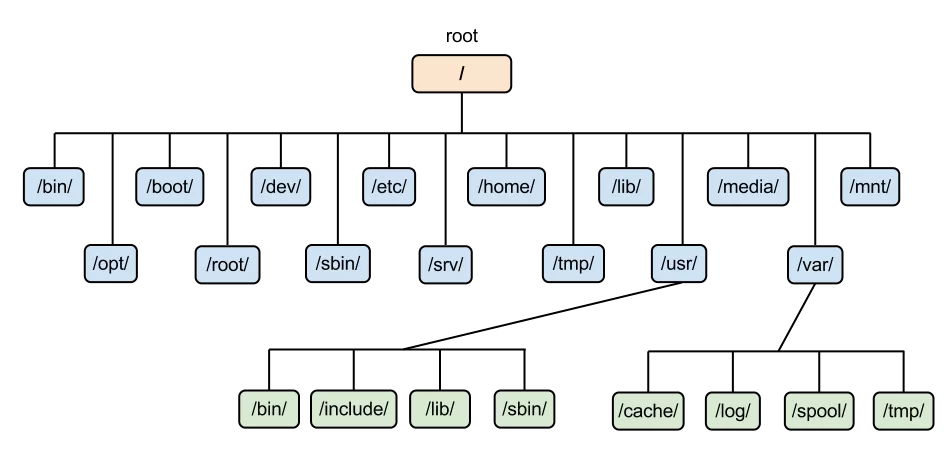
\includegraphics[width=\textwidth]{img/ch1/hfs.png}
	\caption{Иерархия файловой системы}
	\label{fig:galaxy}
\end{figure}

\keystroke{Сtrl + Shift + F}


man -K IPX

\texttt{man}

\keystroke{Сtrl} + \keystroke{Shift} + \keystroke{F}

\section{vi}
\section{nano}
\section{базовые команды}
\section{регулярные выражения}
\section{командая строка и bash}
\section{экранные менеджеры screen, tmux}
